% Options for packages loaded elsewhere
\PassOptionsToPackage{unicode}{hyperref}
\PassOptionsToPackage{hyphens}{url}
%
\documentclass[
  ignorenonframetext,
]{beamer}
\usepackage{pgfpages}
\setbeamertemplate{caption}[numbered]
\setbeamertemplate{caption label separator}{: }
\setbeamercolor{caption name}{fg=normal text.fg}
\beamertemplatenavigationsymbolsempty
% Prevent slide breaks in the middle of a paragraph
\widowpenalties 1 10000
\raggedbottom
\setbeamertemplate{part page}{
  \centering
  \begin{beamercolorbox}[sep=16pt,center]{part title}
    \usebeamerfont{part title}\insertpart\par
  \end{beamercolorbox}
}
\setbeamertemplate{section page}{
  \centering
  \begin{beamercolorbox}[sep=12pt,center]{part title}
    \usebeamerfont{section title}\insertsection\par
  \end{beamercolorbox}
}
\setbeamertemplate{subsection page}{
  \centering
  \begin{beamercolorbox}[sep=8pt,center]{part title}
    \usebeamerfont{subsection title}\insertsubsection\par
  \end{beamercolorbox}
}
\AtBeginPart{
  \frame{\partpage}
}
\AtBeginSection{
  \ifbibliography
  \else
    \frame{\sectionpage}
  \fi
}
\AtBeginSubsection{
  \frame{\subsectionpage}
}
\usepackage{amsmath,amssymb}
\usepackage{lmodern}
\usepackage{ifxetex,ifluatex}
\ifnum 0\ifxetex 1\fi\ifluatex 1\fi=0 % if pdftex
  \usepackage[T1]{fontenc}
  \usepackage[utf8]{inputenc}
  \usepackage{textcomp} % provide euro and other symbols
\else % if luatex or xetex
  \usepackage{unicode-math}
  \defaultfontfeatures{Scale=MatchLowercase}
  \defaultfontfeatures[\rmfamily]{Ligatures=TeX,Scale=1}
\fi
% Use upquote if available, for straight quotes in verbatim environments
\IfFileExists{upquote.sty}{\usepackage{upquote}}{}
\IfFileExists{microtype.sty}{% use microtype if available
  \usepackage[]{microtype}
  \UseMicrotypeSet[protrusion]{basicmath} % disable protrusion for tt fonts
}{}
\makeatletter
\@ifundefined{KOMAClassName}{% if non-KOMA class
  \IfFileExists{parskip.sty}{%
    \usepackage{parskip}
  }{% else
    \setlength{\parindent}{0pt}
    \setlength{\parskip}{6pt plus 2pt minus 1pt}}
}{% if KOMA class
  \KOMAoptions{parskip=half}}
\makeatother
\usepackage{xcolor}
\IfFileExists{xurl.sty}{\usepackage{xurl}}{} % add URL line breaks if available
\IfFileExists{bookmark.sty}{\usepackage{bookmark}}{\usepackage{hyperref}}
\hypersetup{
  pdftitle={Transformation of Microfinance Institutions in Africa},
  pdfauthor={John Karuitha \& Kalu Ojah},
  hidelinks,
  pdfcreator={LaTeX via pandoc}}
\urlstyle{same} % disable monospaced font for URLs
\newif\ifbibliography
\usepackage{graphicx}
\makeatletter
\def\maxwidth{\ifdim\Gin@nat@width>\linewidth\linewidth\else\Gin@nat@width\fi}
\def\maxheight{\ifdim\Gin@nat@height>\textheight\textheight\else\Gin@nat@height\fi}
\makeatother
% Scale images if necessary, so that they will not overflow the page
% margins by default, and it is still possible to overwrite the defaults
% using explicit options in \includegraphics[width, height, ...]{}
\setkeys{Gin}{width=\maxwidth,height=\maxheight,keepaspectratio}
% Set default figure placement to htbp
\makeatletter
\def\fps@figure{htbp}
\makeatother
\setlength{\emergencystretch}{3em} % prevent overfull lines
\providecommand{\tightlist}{%
  \setlength{\itemsep}{0pt}\setlength{\parskip}{0pt}}
\setcounter{secnumdepth}{-\maxdimen} % remove section numbering
\ifluatex
  \usepackage{selnolig}  % disable illegal ligatures
\fi
\newlength{\cslhangindent}
\setlength{\cslhangindent}{1.5em}
\newlength{\csllabelwidth}
\setlength{\csllabelwidth}{3em}
\newenvironment{CSLReferences}[2] % #1 hanging-ident, #2 entry spacing
 {% don't indent paragraphs
  \setlength{\parindent}{0pt}
  % turn on hanging indent if param 1 is 1
  \ifodd #1 \everypar{\setlength{\hangindent}{\cslhangindent}}\ignorespaces\fi
  % set entry spacing
  \ifnum #2 > 0
  \setlength{\parskip}{#2\baselineskip}
  \fi
 }%
 {}
\usepackage{calc}
\newcommand{\CSLBlock}[1]{#1\hfill\break}
\newcommand{\CSLLeftMargin}[1]{\parbox[t]{\csllabelwidth}{#1}}
\newcommand{\CSLRightInline}[1]{\parbox[t]{\linewidth - \csllabelwidth}{#1}\break}
\newcommand{\CSLIndent}[1]{\hspace{\cslhangindent}#1}

\title{\textbf{Transformation of Microfinance Institutions in Africa}}
\subtitle{
\includegraphics[width=3in,height=\textheight]{logo_wits.png}}
\author{\emph{John Karuitha \& Kalu Ojah}}
\date{}

\begin{document}
\frame{\titlepage}

\begin{frame}[fragile]{Background.}
\protect\hypertarget{background.}{}
\begin{itemize}
\item
  For several decades academic researchers and development practitioners
  have hailed \texttt{microfinance} as a key piece in resolving
  financial exclusion and reducing poverty worldwide.
\item
  Traditionally, \texttt{Microfinance\ Institutions\ (MFIs)} have
  operated as non-profit Non-Governmental Organizations (NGOs).
\item
  These NGOs-type MFIs have focused chiefly on availing financial
  services to the financially excluded like women, rural dwellers, and
  the youth.
\end{itemize}
\end{frame}

\begin{frame}{Background: The Paradigm Shift to Profits.}
\protect\hypertarget{background-the-paradigm-shift-to-profits.}{}
\begin{itemize}
\item
  However, MFIs are shifting from the NGO, not-for-profit model of
  microfinance to the commercial, profit-oriented model.
\item
  The shift has especially gained pace with the rise of neo-liberalism
  after the cold war.
\item
  Neo-liberalism emphasizes financial sustainability of economic
  entities, as opposed to reliance on donations and state subsidies, the
  logic behind SAPs.
\end{itemize}
\end{frame}

\begin{frame}[fragile]{Background: Is the Transformation of MFIs that
Bad?}
\protect\hypertarget{background-is-the-transformation-of-mfis-that-bad}{}
\begin{itemize}
\item
  The key concern regarding the paradigm shift is ``Mission drift.''
\item
  Mission drift refers to a scenario where profit-oriented MFIs pay less
  attention to their social mission of availing financial services to
  the financially excluded.
\item
  Instead, profit-maximization takes centre stage.
\item
  Other researchers argue that focus on profits may
  \texttt{erode\ the\ legitimacy} of the microfinance industry, making
  it hard to attract donations and subsidies.
\end{itemize}
\end{frame}

\begin{frame}{Background: Maybe the Conversion of MFIs is Good!}
\protect\hypertarget{background-maybe-the-conversion-of-mfis-is-good}{}
\begin{itemize}
\item
  Other researchers argue that the financial self-sufficiency of MFIs is
  vital for a sustainable microfinance industry.
\item
  Garmaise and Natividad (2013) note that donations to MFIs are
  influenced by the state of bilateral political relationships between
  donor and recipient countries.
\item
  Also, analysis by Armendariz, et al.~(2013) shows that the level of
  donations and subsidies is volatile and heavily influenced by
  macroeconomic factors.
\item
  Kota (2007) argues for the conversion of MFIs, noting that MFIs funded
  via donations and subsidies crowd out viable alternative financial
  intermediaries.
\end{itemize}
\end{frame}

\begin{frame}{Key Research Question}
\protect\hypertarget{key-research-question}{}
\emph{What Drives Microfinance Institutions in Africa to Convert from
NGOs to Commercial Entities?}
\end{frame}

\begin{frame}{Theoretical link}
\protect\hypertarget{theoretical-link}{}
\begin{itemize}
\item
  \textbf{Institutional theory}: Why do organizations change over time
  (DiMaggio and Powell 1991; Martinez-Ferrero and Garcia-Sanchez 2017)?

  \begin{itemize}
  \tightlist
  \item
    The institutional environment dictates change more than market
    pressures.
  \item
    Coercion is a major initiator of change. Donors may push MFIs to
    convert.
  \item
    Change in organizations may arise out of the need to conform to
    institutional environment.
  \end{itemize}
\item
  \textbf{Agency theory}: The social mission of microfinance may
  conflict with the profit motive of finance providers (Jensen and
  Meckling 1976).
\item
  The potential conflict reduce motivation for transformation among
  socially minded donors.
\end{itemize}
\end{frame}

\begin{frame}{Data and variables}
\protect\hypertarget{data-and-variables}{}
\begin{itemize}
\item
  We source panel data from the World Bank's MIX market for 705 MFIs
  operating in 40 African countries.
\item
  Additional data is from the World Development Indicators (WDI) and the
  Worldwide Governance Indicators (WGI) World Bank Databases.
\item
  The panels are unbalanced.
\end{itemize}
\end{frame}

\begin{frame}{Analysis Method}
\protect\hypertarget{analysis-method}{}
\begin{itemize}
\item
  We run mixed effects logit and probit models with NGO type MFIs as the
  base outcome.
\item
  We also incorporate time dummies.
\item
  The model is as follows;
\end{itemize}

\(Y_{it} = \beta_{0} + \beta_{1}X_{it} + \epsilon_{it}\).

for \(Y_{it} = log(\frac{p_{it}}{1 - p_{it}})\).
\end{frame}

\begin{frame}{Analysis Method}
\protect\hypertarget{analysis-method-1}{}
\(p_{it} = \frac{1}{(1 + e^{-z_{it}})}\)

\(1 - p_{it} = \frac{1}{(1 + e^{z_{it}})}\)

\begin{itemize}
\item
  \(p_{it}\) is the probability of an MFI changing from an NGO to any of
  the commercial models.
\item
  \(1 - p_{it}\) is the probability of an NGO remaining an NGO.
\end{itemize}
\end{frame}

\begin{frame}{The Dependent Variable}
\protect\hypertarget{the-dependent-variable}{}
\begin{itemize}
\item
  The current legal status of an MFI is the dependent variable.
\item
  The variable has 5 distinct classes;

  \begin{itemize}
  \tightlist
  \item
    Cooperatives: 1427,
  \item
    NBFIs: 1318,
  \item
    NGO: 1280,
  \item
    Commercial Banks: 619
  \item
    Rural Banks: 138
  \end{itemize}
\item
  NGOs are the base outcome (0). The other classes take a code of 1.
\end{itemize}
\end{frame}

\begin{frame}{The Dependent Variable}
\protect\hypertarget{the-dependent-variable-1}{}
\begin{itemize}
\tightlist
\item
  Dependent variable breakdown
\end{itemize}

\begin{table}

\caption{\label{tab:unnamed-chunk-1}Breakdown of Legal Status of MFIs in Africa}
\centering
\begin{tabular}[t]{ll}
\toprule
Legal\_Status & Number\\
\midrule
NGO & 1280\\
Others & 3502\\
\bottomrule
\multicolumn{2}{l}{\textsuperscript{*} The other legal forms of}\\
\multicolumn{2}{l}{MFIs are cooperatives,}\\
\multicolumn{2}{l}{commercial banks,}\\
\multicolumn{2}{l}{non-bank financial}\\
\multicolumn{2}{l}{institutions, and rural}\\
\multicolumn{2}{l}{banks}\\
\end{tabular}
\end{table}
\end{frame}

\begin{frame}{The Independent variables}
\protect\hypertarget{the-independent-variables}{}
\begin{itemize}
\tightlist
\item
  The following are the independent variables
\item
  MFI Age dummy - New (0 - 4 years), Young (4 - 8 years), and Mature
  (Over 8 years).
\item
  Country Legal tradition dummy - Civil Law, Common Law, and Others.
\item
  Size (the Log of assets). larger MFIs could resist pressure to
  transform.
\item
  Country-level Institutional Quality (Governance)
\end{itemize}
\end{frame}

\begin{frame}{The Independent variables (continued \ldots\ldots.)}
\protect\hypertarget{the-independent-variables-continued-.}{}
\begin{itemize}
\tightlist
\item
  Private Credit to GDP (Reflects banking sector development).
\item
  Stock Market Capitalisation to GDP (Reflects stock market
  development).
\item
  GDP Annual Growth rate (Macroeconomic conditions that may affect fund
  raising).
\end{itemize}
\end{frame}

\begin{frame}{The Independent variables (continued \ldots\ldots.)}
\protect\hypertarget{the-independent-variables-continued-.-1}{}
\begin{figure}
\centering
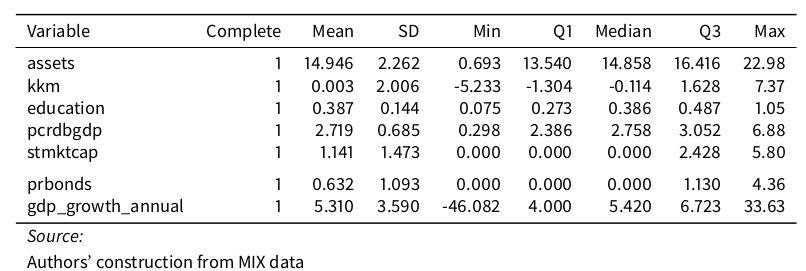
\includegraphics{presentation_shot3.png}
\caption{Independent variables}
\end{figure}
\end{frame}

\begin{frame}{Exploratory data analysis\ldots..}
\protect\hypertarget{exploratory-data-analysis..}{}
\begin{figure}
\centering
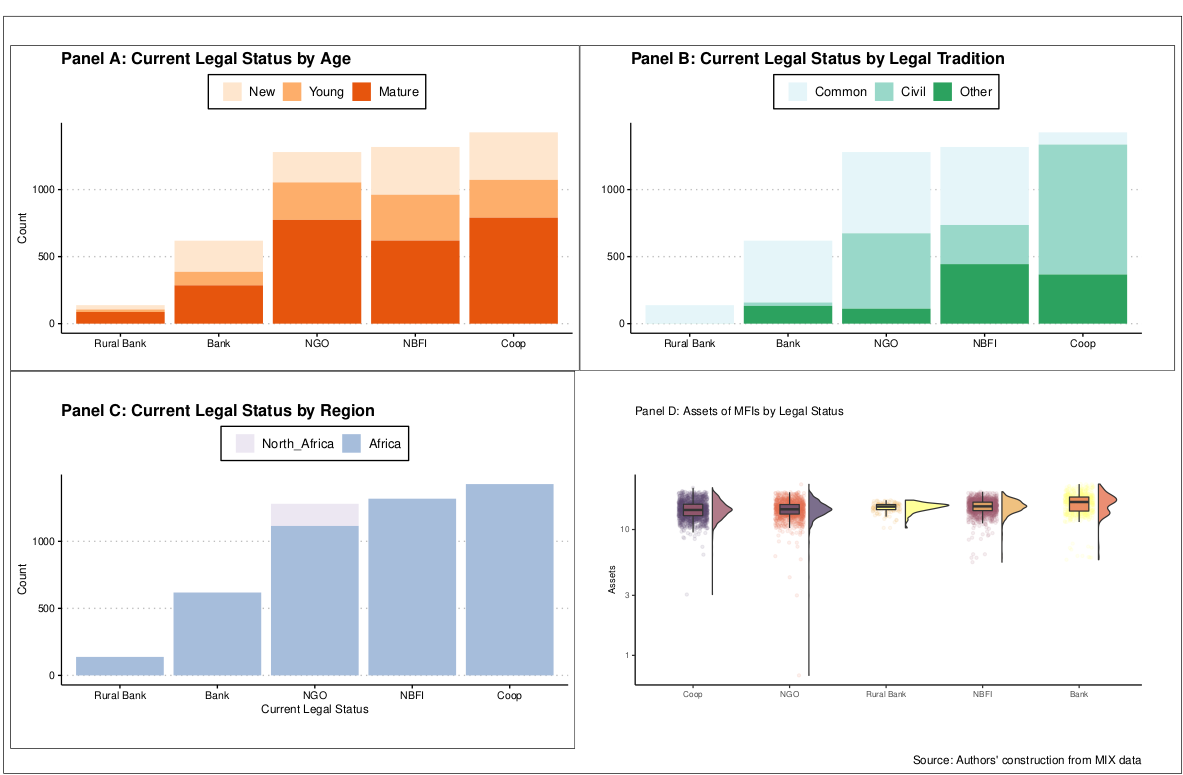
\includegraphics{presentation_shot.png}
\caption{Presentation shot}
\end{figure}
\end{frame}

\begin{frame}{Exploratory data analysis\ldots..}
\protect\hypertarget{exploratory-data-analysis..-1}{}
\begin{figure}
\centering
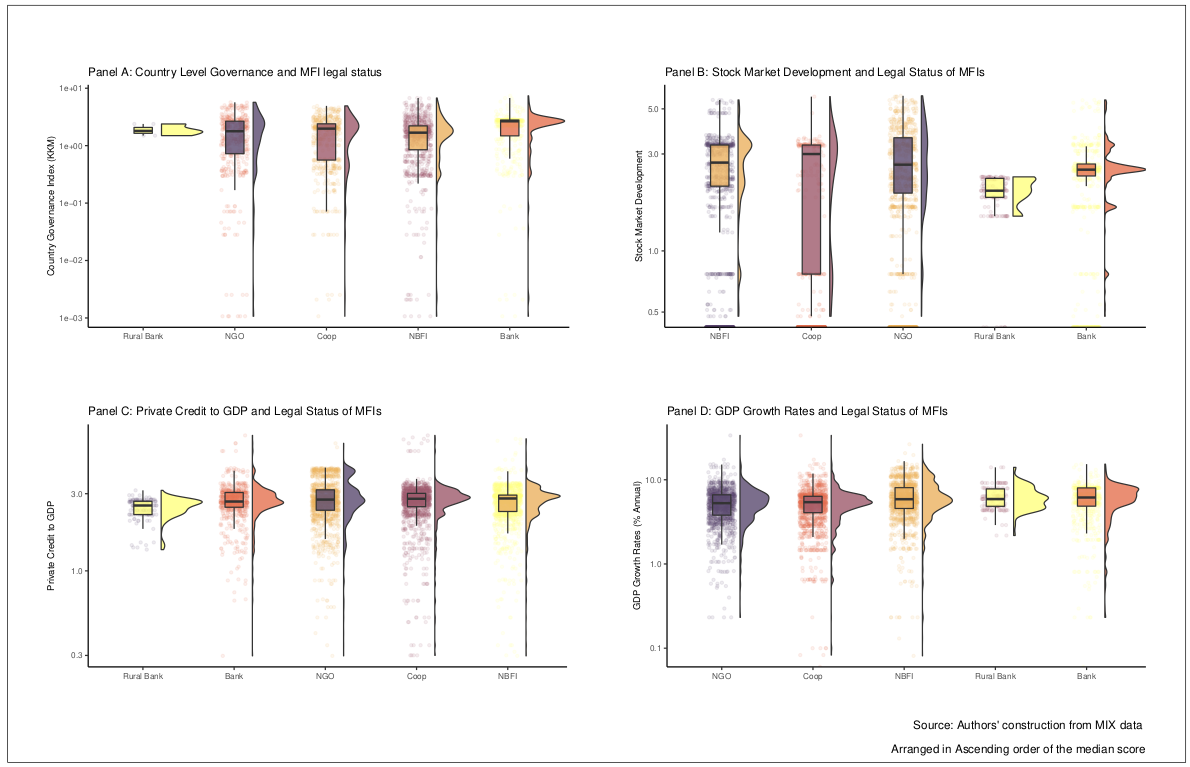
\includegraphics{presentation_shot1.png}
\caption{Presentation shot 1}
\end{figure}
\end{frame}

\begin{frame}{Results of the Regressions}
\protect\hypertarget{results-of-the-regressions}{}
\begin{figure}
\centering
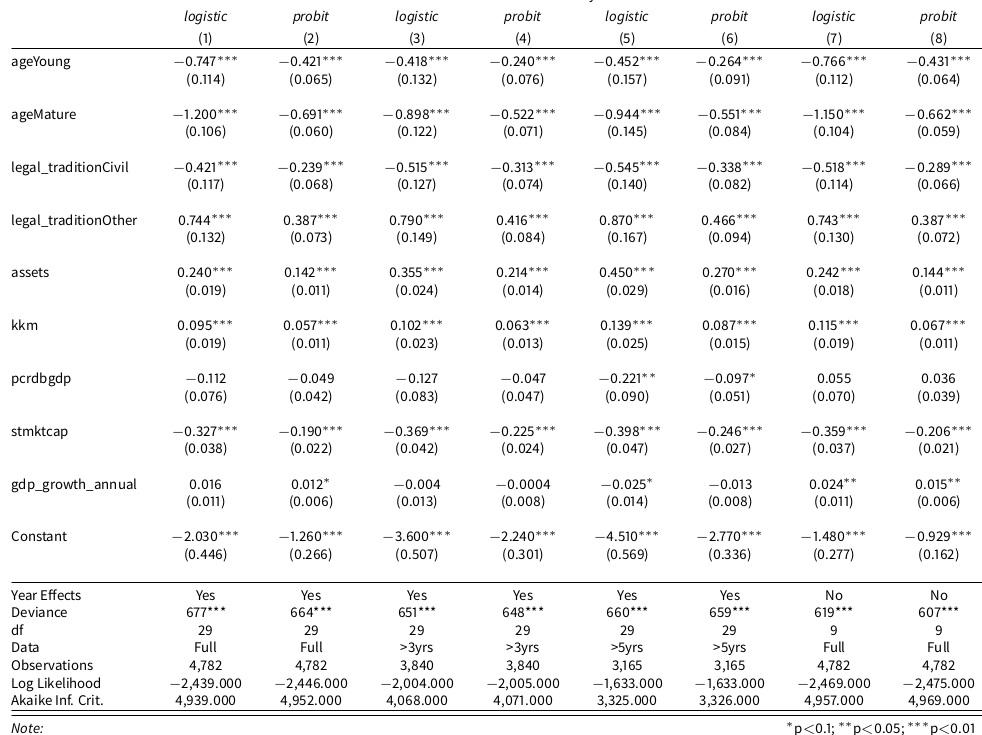
\includegraphics{presentation_shot4.png}
\caption{Regression output}
\end{figure}
\end{frame}

\begin{frame}{Results of the Regressions}
\protect\hypertarget{results-of-the-regressions-1}{}
\begin{itemize}
\item
  The significant drivers of the chance of converting are;

  \begin{itemize}
  \tightlist
  \item
    Age.
  \item
    Size.
  \item
    Legal tradition.
  \item
    Institutional quality, and
  \item
    Stock market development.
  \end{itemize}
\item
  The following variables do not significantly drive transformation;

  \begin{itemize}
  \tightlist
  \item
    Private credit to GDP.
  \item
    GDP growth rate.
  \end{itemize}
\end{itemize}
\end{frame}

\begin{frame}{Results of the Regressions}
\protect\hypertarget{results-of-the-regressions-2}{}
\begin{itemize}
\item
  Age: Mature firms more likely to transform than new or young MFIs,
  likely because they have collateral, goodwill to pledge in return for
  capital markets funding.
\item
  Size: Larger firms more likely to transform, probably because they can
  raise funds easily in capital markets.
\end{itemize}
\end{frame}

\begin{frame}{Results of the Regressions}
\protect\hypertarget{results-of-the-regressions-3}{}
\begin{itemize}
\item
  Legal tradition: MFIs in civil law countries are less likely to
  convert. However, those in other legal traditions are more likely to
  transform.
\item
  MFIs in countries with stronger institutions are more likely to
  transform, likely due to ease of contract enforcement and property
  rights.
\item
  Stronger stock markets correspond with lower chances of
  transformation. If a country has strong capital markets, it is likely
  to have less financial exclusion, hence low demand for microfinance.
\end{itemize}
\end{frame}

\begin{frame}{Results of the Regressions (Insignificant variables)}
\protect\hypertarget{results-of-the-regressions-insignificant-variables}{}
\begin{itemize}
\item
  Stronger private credit markets correspond with lower chances of
  transformation.
\item
  Like for stock markets, if a country has strong credit markets, it is
  likely to have less financial exclusion, hence low demand for
  microfinance.
\end{itemize}
\end{frame}

\begin{frame}{Robustness tests}
\protect\hypertarget{robustness-tests}{}
\begin{itemize}
\item
  We ran the following robustness checks;

  \begin{itemize}
  \item
    We removed outliers and ran the logit and probit models.
  \item
    We also ran multinomial logit model.
  \item
    Checked for multicollinearity and linearity of variables.
  \end{itemize}
\end{itemize}
\end{frame}

\begin{frame}{Conclusion}
\protect\hypertarget{conclusion}{}
\begin{itemize}
\item
  Age and size are the key drivers of MFIs transformation.
\item
  Legal tradition, institutional quality, and stock market
  capitalisation also influence transformation.
\item
  Policy targeting small MFIs to have ample quality assets would enhance
  the chances of transformation.
\end{itemize}
\end{frame}

\begin{frame}{Selected References}
\protect\hypertarget{selected-references}{}
\hypertarget{refs}{}
\begin{CSLReferences}{1}{0}
\leavevmode\hypertarget{ref-maggio1991}{}%
DiMaggio, P., and W. Powell. 1991. {``Introduction.''} In \emph{The New
Institutionalism and Organizational Analysis}, 1--38. University of
Chicago Press.

\leavevmode\hypertarget{ref-jensen1976theory}{}%
Jensen, Michael C, and William H Meckling. 1976. {``Theory of the Firm:
Managerial Behavior, Agency Costs and Ownership Structure.''}
\emph{Journal of Financial Economics} 3 (4): 305--60.

\leavevmode\hypertarget{ref-martinez2017coercive}{}%
Martinez-Ferrero, Jennifer, and Isabel-Maria Garcia-Sanchez. 2017.
{``Coercive, Normative and Mimetic Isomorphism as Determinants of the
Voluntary Assurance of Sustainability Reports.''} \emph{International
Business Review} 26 (1): 102--18.

\end{CSLReferences}
\end{frame}

\end{document}
